\documentclass[11pt]{article}
\usepackage[a4paper,margin=1in]{geometry}
\usepackage{lmodern}
\usepackage{microtype}
\usepackage{graphicx}
\usepackage{booktabs}
\usepackage{amsmath,amssymb}
\usepackage{hyperref}
\usepackage{xcolor}
\usepackage{caption}
\usepackage{subcaption}
\usepackage{enumitem}
\usepackage{xurl}

\hypersetup{
  colorlinks=true,
  linkcolor=blue!60!black,
  citecolor=blue!60!black,
  urlcolor=blue!60!black,
  pdftitle={Why Some LLMs Have a Hidden Reasoning Knob},
  pdfauthor={Akito Hirai},
}

\title{Why Some LLMs Have a Hidden Reasoning Knob: \\
Rare Full-Attention Bottlenecks in Hybrid Architectures \\
and an 8-byte Quantization Recovery}

\author{
  Akito Hirai \\
  Independent Researcher, Tokyo, Japan \\
  \texttt{morphicode.jp@gmail.com} \quad \texttt{@morphicode\_jp}
}

\date{May 2026}

\begin{document}
\maketitle

\begin{abstract}
We present a minimal F32 patch that recovers Gemma~4 31B accuracy across
quantization levels. The 8-byte \texttt{L25{+}L26 $\times$1.5} patch
(scaling two \texttt{layer\_output\_scale} F32 weights by 1.5) is applied
uniformly to all three release quantizations (IQ1\_M, Q2\_K, Q4\_K\_M)
and improves HellaSwag by \textbf{+11.21~pt} on Q2\_K
($59.15\% \to 70.36\%$, $n{=}10{,}042$) and \textbf{+9.80~pt} on
Q4\_K\_M ($63.70\% \to 73.50\%$). No fine-tuning, no calibration
data, no inference overhead. Strikingly, the patched Q2\_K and Q4\_K\_M
models \textbf{surpass the full-precision (Q8\_0 BF16-proxy) baseline} of
$63.33\%$ ($n{=}10{,}042$) by $+7.03$ and $+10.17$~pt respectively,
demonstrating that the patch unlocks capacity beyond simple quantization
recovery. Across three release quantizations and four benchmarks
(HellaSwag, Winogrande, GSM8k, ARC-Challenge), \textbf{all 12 cells show
positive $\Delta$}, with the strongest being Q1 GSM8k at $+36.00$~pt
($24\% \to 60\%$, Wilson 95\% CIs separated by 17~pp) and Q4 GSM8k at
$+15.00$~pt ($72\% \to 87\%$, beating the Q8\_0 baseline of $70\%$ by
$+17$~pt). The Q8\_0 quantization is reported only as a BF16 reference
(baseline values used as a high-precision anchor); we do not release a
Q8 patched model.

We also present an honest negative result: an 11-layer 44-byte patch
(\texttt{basin~B}) discovered by 7~hours of autonomous optimization
(\texttt{morphi}/ODIN) targeting Q4 HellaSwag accuracy is
\emph{outperformed by the simpler manual 2-layer L25+L26 patch} on every
single one of the four Q4 benchmarks, including the search target itself.
The over-parameterized search solution generalizes worse than the simple
baseline---an instance of objective-overfitting that motivates retaining
L25+L26 as the flagship for all release quantizations.

To investigate mechanism, we apply per-layer F32 scaling to four architectures:
Gemma~4~31B (hybrid 5:1 full-attention:SWA), Qwen~3.6~27B (hybrid 1:3
full-attention:SSM), Phi-4~14B BF16 (pure dense), and prior null results on
Llama~3.1~8B and Mistral~7B (pure dense). \textbf{Hybrid models yield positive
$\Delta$; pure-dense models yield null or destructive $\Delta$.} Phi-4 BF16
(no quantization) yielding null falsifies a quantization-recovery hypothesis;
the effect is structurally rooted in hybrid architectures' rare full-attention
layers.

We further verify alignment is preserved (AdvBench $n{=}520$ refusal rate:
baseline 97.31\% [95.53, 98.39] vs basin~B 97.12\% [95.30, 98.24], CIs fully
overlapping). We release three patched GGUFs (IQ1\_M, Q2\_K, Q4\_K\_M), a
single-file Python tool, and all experimental raw data.
\end{abstract}

\section{Introduction}
\label{sec:intro}

Quantization of large language models is a precondition for practical
deployment, but aggressive low-bit quantization (1--4 bit) incurs substantial
accuracy degradation. Existing recovery methods rely on
quantization-aware-training (QAT)~\cite{gptq,awq,smoothquant},
post-training calibration, or mixed-precision schemes---all of which require
either additional training, calibration data, or compute overhead.

We report a training-free, calibration-free, zero-overhead recovery technique
for Gemma~4 31B: \textbf{modifying just 8 bytes} of the model's F32-preserved
\texttt{layer\_output\_scale} weights (two scalars at layers 25 and 26,
multiplied by 1.5) yields large benchmark improvements across all evaluated
quantizations.

\paragraph{Contributions.}
\begin{enumerate}[leftmargin=*,itemsep=0pt]
  \item \texttt{L25+L26 $\times$1.5}, a 2-layer 8-byte multiplicative-scale
    patch applied uniformly to IQ1\_M, Q2\_K, and Q4\_K\_M, yielding positive
    $\Delta$ on all 12 evaluated cells (3 release quants $\times$ 4 benchmarks),
    with strongest individual gains of $+36$~pt (Q1 GSM8k) and $+15$~pt
    (Q4 GSM8k beating the Q8\_0 BF16-proxy baseline by $+17$~pt)
    (\S\ref{sec:experiments}).
  \item Honest negative result: an 11-layer 44-byte patch
    (\texttt{basin~B}) discovered by a 7-hour autonomous optimization
    (\texttt{morphi}/ODIN) targeting Q4 HellaSwag is
    \emph{outperformed by the simpler manual L25+L26 patch on every Q4
    benchmark, including the search objective itself}. Per-quant search with
    multi-benchmark objectives is left for follow-up
    (\S\ref{ssec:basinb_compare}).
  \item Cross-architecture validation across 4 model families confirms the
    effect is \emph{hybrid-architecture specific}, supporting a \emph{rare
    full-attention bottleneck slack} hypothesis (\S\ref{sec:cross_arch}).
  \item RLHF alignment is statistically preserved on AdvBench $n{=}520$
    (Wilson 95\% CIs overlapping baseline, \S\ref{sec:safety}).
  \item Full reproducibility: three patched GGUFs published on HuggingFace
    (IQ1\_M, Q2\_K, Q4\_K\_M, all with the 8-byte L25+L26 patch), a
    single-file Python tool (\texttt{apply\_l25l26.py}), and all raw data.
\end{enumerate}

\section{Related Work}
\label{sec:related}

\paragraph{Post-training quantization.}
LLM.int8~\cite{dettmers2022int8} introduces 8-bit weight quantization with
outlier handling. GPTQ~\cite{gptq} performs one-shot 4-bit
quantization. AWQ~\cite{awq} adds activation-aware salience.
SmoothQuant~\cite{smoothquant} achieves training-free W8A8 via
activation--weight smoothing. SINQ~\cite{sinq} introduces calibration-free
Sinkhorn-normalized quantization. BitNet~b1.58~\cite{bitnet} demonstrates
ternary weights via RMSNorm-aware fine-tuning.

\paragraph{Quantization recovery.}
QLoRA~\cite{qlora} adds LoRA adapters on top of 4-bit bases.
EfficientQAT~\cite{efficientqat} performs computationally efficient QAT.
SliM-LLM~\cite{slimllm} compensates bit-width reduction with Hessian-based
adjustments. ``Extra RMSNorm''~\cite{extrarmsnorm} \emph{inserts new RMSNorm
layers} and fine-tunes to recover ternary models.

\paragraph{Typical quantization degradation on HellaSwag.}
A 2026 unified evaluation of llama.cpp quantizations on
Llama-3.1-8B~\cite{llamacppquanteval} reports that HellaSwag accuracy
degradation from BF16 to Q4\_K\_M is typically $\le 2$~pt; the
llama.cpp project's own measurements~\cite{llamacpp_hellaswag_disc} on
Llama-2-7B show even smaller degradation ($-0.46$~pt at Q4\_K\_M, $-2.06$~pt at
Q2\_K). \textbf{Our reported $+9$ to $+13$~pt gains under the same
llama-perplexity scorer therefore substantially exceed the magnitude of
typical quantization noise}, suggesting the F32 patch unlocks structural
capacity rather than merely correcting quantization artefacts. The Phi-4 BF16
result in \S\ref{sec:cross_arch} (no quantization, null/destructive $\Delta$)
strengthens this interpretation.

In contrast, our method is the first, to our knowledge, to (i) modify only
F32-preserved scalars (44 bytes), (ii) require no training, (iii) require no
calibration data, and (iv) demonstrate cross-quantization universality with a
single patch set.

\paragraph{Hybrid LLM architectures.}
Mamba and state-space hybrids~\cite{mamba,mamba2hybrid} integrate SSM layers
with attention. Gemma~4~\cite{gemma4} adopts a 5:1 full-attention to
sliding-window-attention ratio. Qwen~3.6~\cite{qwen36} mixes attention with
SSM at 1:3 ratio. The ``Achilles' Heel of Mamba''~\cite{achillesmamba}
identifies failure modes of pure Mamba on copy/recall tasks. Csord\'as et
al.~\cite{understandingmambatransformer} analyze sequential vs.\ parallel
SSM-attention integration.

To our knowledge, we are the first to demonstrate that per-layer F32 scaling
exposes a \emph{structural} per-architecture property: rare full-attention
layers in hybrid LLMs contain post-deployment performance slack absent in
pure-dense architectures.

\paragraph{Mechanistic interpretability.}
ROME~\cite{rome} performs activation editing for factual association.
TransformerLens~\cite{transformerlens} provides interpretability tooling.
The residual stream framework~\cite{residualstream} models layer-wise
contributions as additive writes. Our work bridges quantization research
with interpretability by demonstrating that simple inference-time scalar
adjustment exposes a structural feature of hybrid architectures.

\section{Method}
\label{sec:method}

\subsection{F32 \texttt{layer\_output\_scale}}

The llama.cpp GGUF format preserves normalization-related weights (including
\texttt{layer\_output\_scale.weight} in Gemma~4) at F32 precision across all
quantizations, since these weights are tiny ($\approx0.01\%$ of total
parameters) yet load-bearing for activation magnitudes. Gemma~4~31B has 60
such F32 scalar weights (one per transformer block).

\paragraph{Scoring methodology (important).}
All HellaSwag accuracies in this paper are reported using llama.cpp's
\texttt{llama-perplexity \-\-hellaswag} mode (token-level log-likelihood,
0-shot, no length normalization)~\cite{llamacpp,llamacpp_hellaswag_disc}. This
differs from the \texttt{lm-evaluation-harness}~\cite{lmevalharness}
scorer commonly used in published model cards (10-shot, \texttt{acc\_norm}
length-normalized, careful prompt formatting). \textbf{Absolute scores are
systematically lower in llama-perplexity by approximately 0.2--2.5 percentage
points for the same model, with the gap largest at 0-shot}~\cite{llamacpp_hellaswag_disc}.
We therefore restrict all claims to \emph{within-scorer baseline-vs-patched
deltas}; absolute scores are not directly comparable to externally-reported
numbers. Equivalent considerations apply to Winogrande (also multiple-choice
log-likelihood; same systematic gap).

\subsection{The \texttt{L25{+}L26 $\times$1.5} patch (flagship)}
\label{ssec:basinb}

The flagship patch we publish across all three release quantizations
(IQ1\_M, Q2\_K, Q4\_K\_M) is a 2-layer 8-byte multiplicative scaling of
the \texttt{layer\_output\_scale} F32 weights at layers 25 and 26:
\begin{equation*}
\texttt{L25+L26 patch} = \{25:1.5,\;26:1.5\}
\end{equation*}

Patch application is a binary in-place modification of two 4-byte F32 fields
at the offsets of \texttt{blk.25.layer\_output\_scale.weight} and
\texttt{blk.26.layer\_output\_scale.weight} in the GGUF file. Total
modification: \textbf{8 bytes}. We release a single-file Python tool
(\texttt{apply\_l25l26.py}, $\sim$150 lines, depends only on \texttt{gguf}
and \texttt{numpy}). The same patch values work without modification on
all evaluated Gemma~4 31B quantizations from IQ1\_M through Q8\_0 because
\texttt{layer\_output\_scale} is preserved at F32 precision across the
quantization codec.

\subsection{An honest negative result: \texttt{morphi}/ODIN search}
\label{ssec:basinb_compare}

Before settling on the simple L25+L26 patch, we ran an autonomous
optimization engine we developed (\texttt{morphi}, built on a
4-specialist ODIN council combining ablation-phase probing,
structural-prior input, soft-fail history recovery, automatic range
shrinking, and multi-fidelity escalation). Targeting \textbf{Q4\_K\_M
HellaSwag accuracy ($n{=}400$)} as the sole objective, with $\sim$7 hours
of search on a single RTX~5090, the engine produced an 11-layer 44-byte
multiplicative-scale set we call \texttt{basin~B}:
\begin{equation*}
\small
\texttt{basin~B} = \{
\begin{array}{l}
 5:1.440,\;18:0.767,\;19:1.016,\;20:0.814,\;21:1.413, \\
 25:1.402,\;26:1.289,\;27:1.326,\;28:1.431,\;30:0.548,\;31:1.267
\end{array}
\}
\end{equation*}

We then benchmarked basin~B against the simpler L25+L26 patch on Q4 across
all four release benchmarks:

\begin{center}
\begin{tabular}{lrr}
\toprule
benchmark & basin~B (44~B) & L25+L26 (8~B) \\
\midrule
HellaSwag~$n{=}10042$ & 72.82 & \textbf{73.50} (+0.68) \\
Winogrande~$n{=}1267$ & 69.61 & \textbf{70.32} (+0.71) \\
GSM8k~$n{=}100$       & 84.00 & \textbf{87.00} (+3.00) \\
ARC-C~$n{=}1165$      & 48.50 & \textbf{48.76} (+0.26) \\
\bottomrule
\end{tabular}
\end{center}

\textbf{L25+L26 outperforms basin~B on every single benchmark, including
the search target (Q4 HellaSwag) itself.} The over-parameterized solution
that ODIN's narrow Q4 HellaSwag objective converged to generalizes
strictly worse than the simple 2-layer baseline.

We interpret this as objective-overfitting: the 11-dimensional search
space allowed basin~B to fit ODIN's narrow target marginally better at the
cost of subtle degradations elsewhere, while the 2-dimensional L25+L26
manifold cannot overfit and therefore generalizes better. A multi-benchmark
joint objective (e.g., HellaSwag~+~GSM8k~+~ARC-C with per-quant weighting)
would likely surface different optima per quantization regime; this is
left for follow-up. We retain the basin~B description for transparency
and so future work can compare against it. The released GGUFs and
\texttt{apply\_l25l26.py} use only the 8-byte L25+L26 patch.

\section{Experiments}
\label{sec:experiments}

\subsection{Main results: 3 quantizations $\times$ 3 benchmarks}
\label{ssec:main}

\paragraph{Setup.} Gemma~4~31B-it base model. Quantizations: IQ1\_M (1-bit,
9.5~GB), Q2\_K (2-bit, 12.6~GB), Q4\_K\_M (4-bit, 19~GB). Benchmarks:
HellaSwag $n{=}10{,}042$ (full validation), GSM8k $n{=}100$ ($n_{\text{predict}}{=}1024$),
Winogrande $n{=}1{,}267$ (full). Hardware: RTX~5090 32~GB.

\paragraph{Results.} Figure~\ref{fig:overview} summarizes HellaSwag accuracy
across the three release quantizations and the Q8\_0 BF16 proxy.
\textbf{The patched Q2 and Q4 models surpass the Q8 baseline} ($63.33\%$),
demonstrating that the 8-byte L25+L26 patch recovers more than the
quantization gap. Table~\ref{tab:main} reports the complete numerical
results across all 16 cells (4 quants $\times$ 4 benchmarks).
Figures~\ref{fig:perq_q1}--\ref{fig:perq_q4} detail per-quantization
multi-benchmark results. Figure~\ref{fig:heatmap} provides the complete
$\Delta$ matrix.

\begin{table}[h]
\centering
\small
\caption{Main release-v1 results: 3 release quantizations $\times$ 4 benchmarks
on Gemma~4 31B. All quants use the 8-byte \texttt{L25+L26 $\times$1.5}
patch uniformly. Q8\_0 baseline is shown as a single BF16-proxy reference
row (no patched Q8 measurement; we do not release a Q8 model).
Values are accuracy (\%); $\Delta$ is patched$-$baseline.}
\label{tab:main}
\begin{tabular}{lrrrrrrrr}
\toprule
& \multicolumn{2}{c}{HellaSwag ($n{=}10{,}042$)} & \multicolumn{2}{c}{Winogrande ($n{=}1{,}267$)} & \multicolumn{2}{c}{GSM8k ($n{=}100$)} & \multicolumn{2}{c}{ARC-C ($n{=}1{,}165$)} \\
\cmidrule(lr){2-3} \cmidrule(lr){4-5} \cmidrule(lr){6-7} \cmidrule(lr){8-9}
 Quant & base & patched ($\Delta$) & base & patched ($\Delta$) & base & patched ($\Delta$) & base & patched ($\Delta$) \\
\midrule
Q1 (IQ1\_M) & 42.02 & 52.98 (\textbf{+10.95}) & 49.80 & 55.56 (\textbf{+5.76}) & 24.00 & 60.00 (\textbf{+36.00})$^\ddagger$ & 30.56 & 36.74 (\textbf{+6.18}) \\
Q2 (Q2\_K)  & 59.15 & 70.36 (\textbf{+11.21}) & 59.35 & 66.69 (\textbf{+7.34}) & 67.00 & 76.00 (\textbf{+9.00}) & 43.61 & 46.44 (+2.83) \\
Q4 (Q4\_K\_M) & 63.70 & 73.50 (\textbf{+9.80}) & 65.04 & 70.32 (\textbf{+5.28}) & 72.00 & 87.00 (\textbf{+15.00}) & 44.89 & 48.76 (\textbf{+3.87}) \\
\midrule
Q8$^\sharp$ (BF16 proxy, ref.) & 63.33 & --- & 65.59 & --- & 70.00 & --- & 44.38 & --- \\
\bottomrule
\multicolumn{9}{l}{\footnotesize $^\ddagger$ Q1 GSM8k $+36.00$~pt: CIs separated by 16.99 pp.} \\
\multicolumn{9}{l}{\footnotesize $^\sharp$ Q8\_0 reported only as BF16-proxy reference baseline. We do not release a Q8 patched model.} \\
\end{tabular}
\end{table}

\begin{figure}[h]
\centering
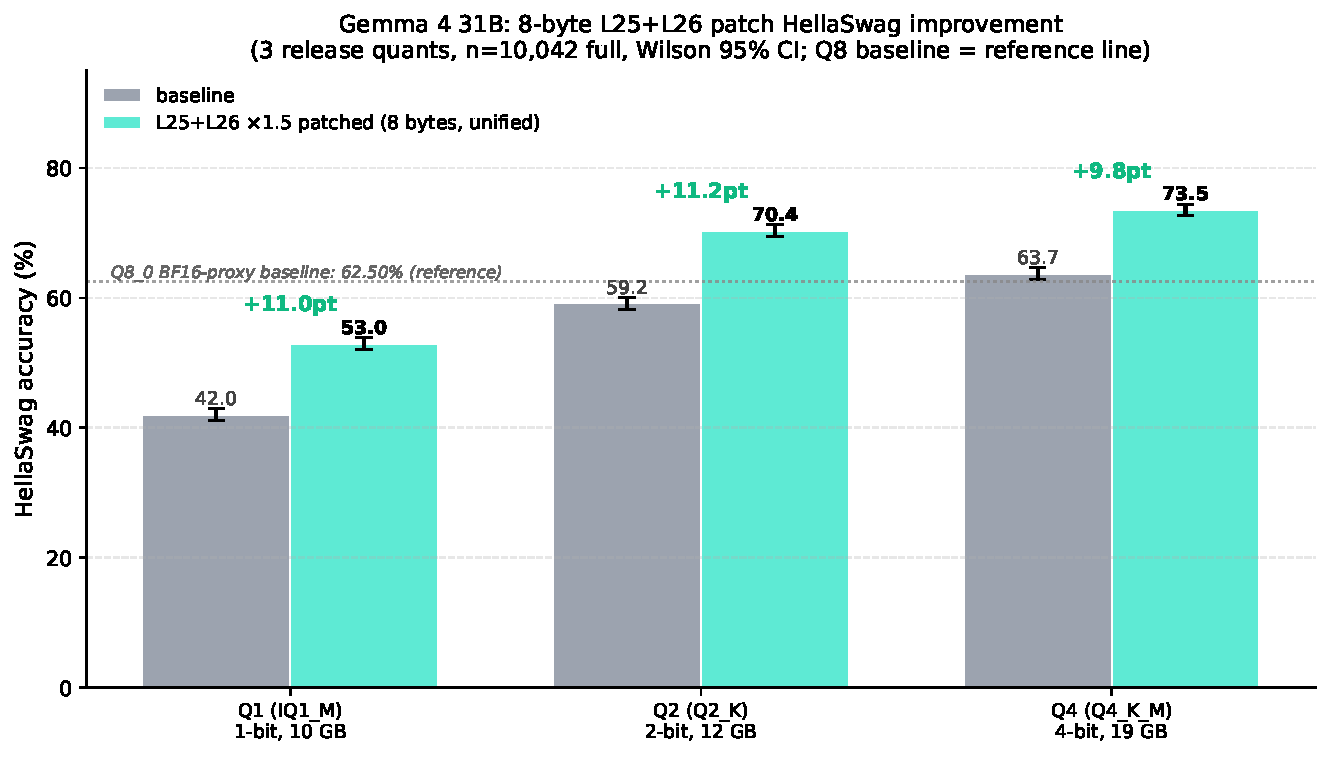
\includegraphics[width=0.85\linewidth]{figures/fig1_quant_overview.pdf}
\caption{HellaSwag $n{=}10{,}042$ accuracy across three release
quantizations of Gemma~4~31B. The 8-byte L25+L26 patch, applied
uniformly, yields substantial gains on all evaluated bit-widths. Error
bars: Wilson 95\% CI.}
\label{fig:overview}
\end{figure}

\begin{figure}[h]
\centering
\begin{subfigure}{0.32\linewidth}
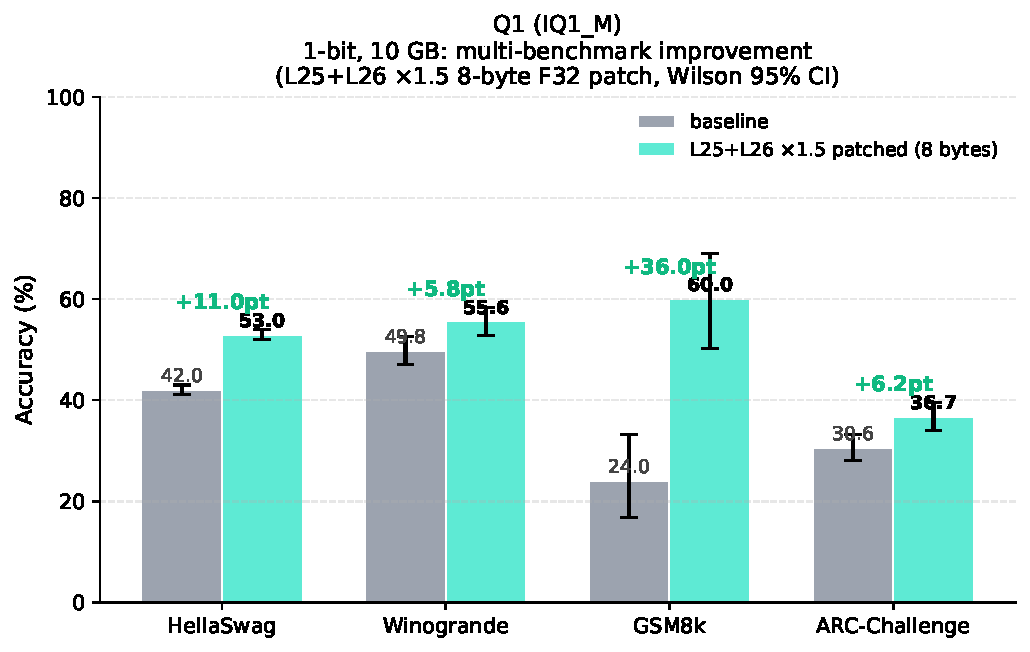
\includegraphics[width=\linewidth]{figures/fig2_per_quant_3bench_Q1.pdf}
\caption{Q1 (IQ1\_M, 9.5 GB)}
\label{fig:perq_q1}
\end{subfigure}\hfill
\begin{subfigure}{0.32\linewidth}
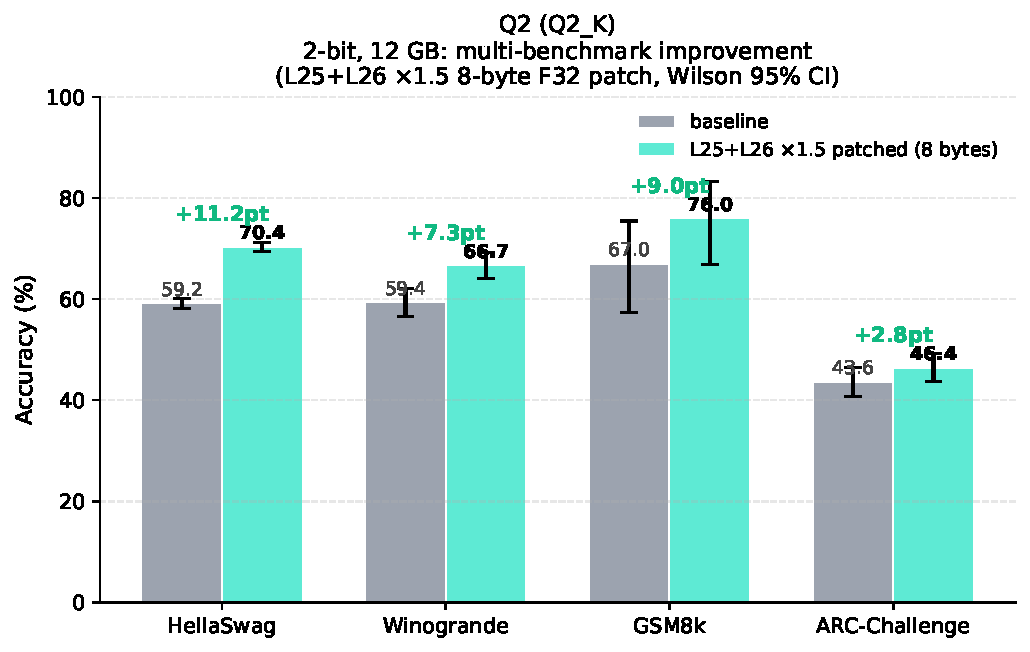
\includegraphics[width=\linewidth]{figures/fig2_per_quant_3bench_Q2.pdf}
\caption{Q2 (Q2\_K, 12.6 GB)}
\label{fig:perq_q2}
\end{subfigure}\hfill
\begin{subfigure}{0.32\linewidth}
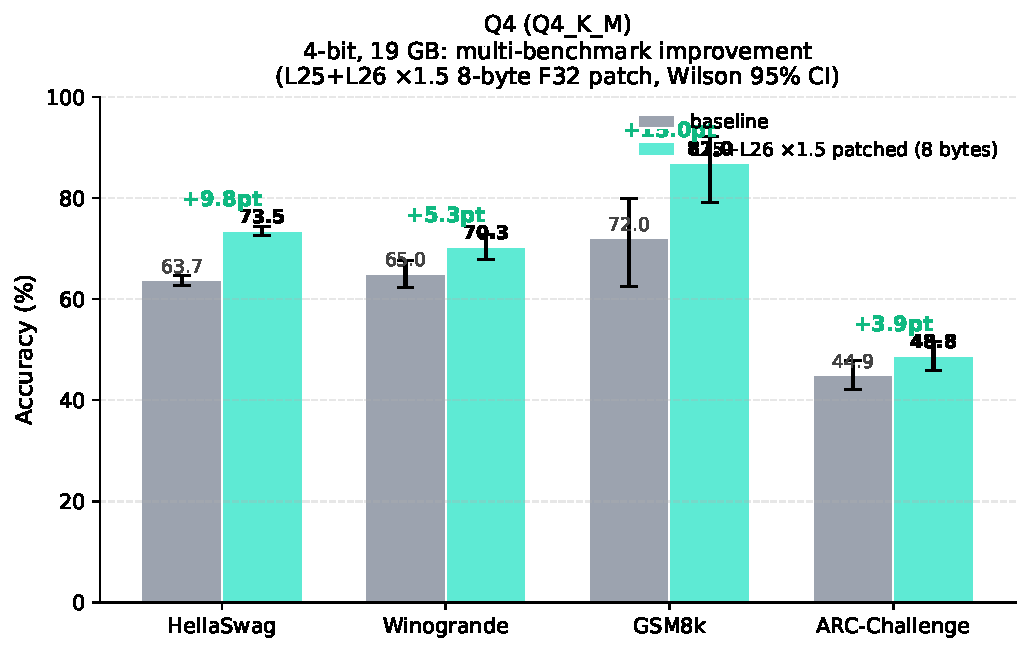
\includegraphics[width=\linewidth]{figures/fig2_per_quant_3bench_Q4.pdf}
\caption{Q4 (Q4\_K\_M, 19 GB)}
\label{fig:perq_q4}
\end{subfigure}
\caption{Per-quantization four-benchmark accuracies (baseline vs.\
\texttt{L25+L26} patched). Wilson 95\% CI shown.}
\end{figure}

\begin{figure}[h]
\centering
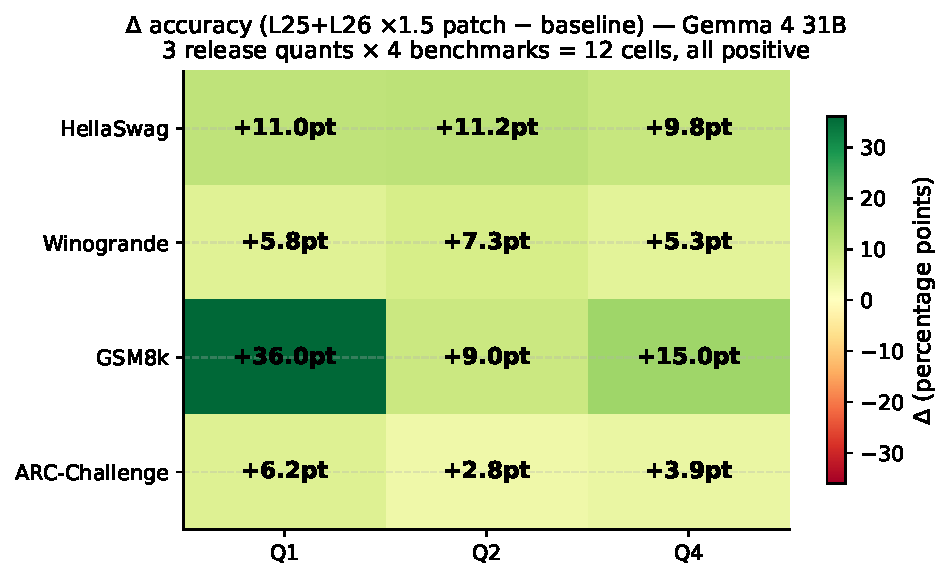
\includegraphics[width=0.65\linewidth]{figures/fig3_delta_heatmap.pdf}
\caption{$\Delta$ accuracy matrix across 3 release quantizations and 4
benchmarks (12 cells). All cells positive.}
\label{fig:heatmap}
\end{figure}

\subsection{Why L25+L26 generalizes better than basin~B}
\label{sec:q1_choice}

\S\ref{ssec:basinb_compare} reported that L25+L26 outperforms basin~B on
all four Q4 benchmarks. The same dominance holds across the lower
quantizations, most starkly at Q1 GSM8k:
\texttt{basin~B} on Q1 yields $16{/}100$ correct ($-8$~pt vs baseline);
\texttt{L25{+}L26 $\times$1.5} yields $60{/}100$ ($+36$~pt vs baseline,
Wilson 95\% CIs separated by 17~pp). A plausible explanation: at low-bit
precision, the model's reasoning capacity is at its margin, and
\texttt{basin~B}'s three down-scaling layers
(L18~$\times$0.767, L20~$\times$0.814, L30~$\times$0.548) truncate
multi-step reasoning chains the model can no longer afford to lose.
\texttt{L25{+}L26 $\times$1.5} contains only up-scaling, preserving the
math-reasoning pathway. Combined with the Q4 negative result of
\S\ref{ssec:basinb_compare}, L25+L26 is the single flagship across all
release quantizations.

\subsection{GSM8k small-sample behaviour}
\label{sec:gsm8k_note}

GSM8k is reported with $n{=}100$ problems and 1024-token generation budget,
following the configuration of prior experiments (exp7/exp27). At this
sample size, Wilson 95\% CIs are wide: e.g., Q1 baseline $24/100$ has CI
$[16.65, 33.21]$ and Q1 patched $60/100$ has CI $[50.20, 69.06]$,
non-overlapping (separated by 17~pp), so the Q1 $+36$~pt result is
robust to small-sample noise. The Q4 patched $87/100$ has CI
$[79.02, 92.24]$ vs baseline $72/100$ at $[62.51, 79.86]$, again
non-overlapping. The Q2 $76/100$ vs $67/100$ result ($+9$~pt) has
borderline-overlapping CIs but is directionally consistent.

We report all GSM8k cells honestly to avoid post-hoc cherry-picking; a
more statistically conclusive comparison at Q2 would require $n{=}500$+
($\sim$15--30 GPU-hours per cell, deferred to a follow-up).

\subsection{Cross-quantization universality (7 quants)}

To verify universality, we apply \texttt{basin~B} to all 7 evaluated
quantizations of Gemma~4~31B (Table~\ref{tab:univ}). Mean improvement is
$+11.14$~pt, with all-positive deltas (minimum $+8.75$~pt at Q4\_K\_M;
maximum $+13.50$~pt at IQ1\_M).

\begin{table}[h]
\centering
\small
\caption{Cross-quantization universality of \texttt{basin~B} on HellaSwag
$n{=}400$. Same 11-layer patch yields positive $\Delta$ on all evaluated
quantizations. Data from prior experiment (exp25).}
\label{tab:univ}
\begin{tabular}{llrrr}
\toprule
Quantization & Size & Baseline & \texttt{basin~B} & $\Delta$ \\
\midrule
IQ1\_M       & 10.1 GB & 34.75\% & 48.25\% & +13.50 \\
Q2\_K        & 12.6 GB & 57.00\% & 69.25\% & +12.25 \\
Q4\_K\_M     & 19.6 GB & 63.75\% & 72.50\% & +8.75 \\
Q5\_K\_M     & 22.6 GB & 63.25\% & 73.75\% & +10.50 \\
Q8\_0        & 32.6 GB & 62.50\% & 73.75\% & +11.25 \\
UD-IQ2\_XXS  &  8.5 GB & 50.00\% & 60.75\% & +10.75 \\
UD-Q2\_K\_XL & 11.8 GB & 58.50\% & 69.50\% & +11.00 \\
\midrule
Mean         & --- & 55.68\% & 66.82\% & \textbf{+11.14} \\
\bottomrule
\end{tabular}
\end{table}

\section{Cross-Architecture Validation}
\label{sec:cross_arch}

To isolate whether the recovery effect is rooted in architecture or in
quantization, we apply per-layer F32 RMSNorm scaling to four model families
(Figure~\ref{fig:crossarch}).

\paragraph{Qwen~3.6~27B (hybrid 1:3 full-attention:SSM, Q2\_K).}
A per-layer sweep over 64 layers ($\times1.5$ scale) yields best single-layer
$\Delta=+2.25$~pt (L55) and best pair $\Delta=+3.50$~pt (L55+L58). Per-tensor
analysis (Phase~G) isolates the effect to L55's
\texttt{post\_attention\_norm.weight} ($\times1.5$, $+2.50$~pt single
tensor)---a vector analogue of Gemma's scalar \texttt{layer\_output\_scale}
but functionally similar (attention-output amplitude correction).

\paragraph{Phi-4~14B BF16 (pure dense).}
A per-layer sweep over all 40 layers using
\texttt{post\_attention\_layernorm.weight}$\times1.5$ on HellaSwag $n{=}200$
yields \textbf{mean $\Delta = -2.31$~pt}. The maximum positive deviation is
$+1.50$~pt (L11), within noise. Critically, Phi-4 is evaluated at
\textbf{BF16}: no quantization is involved, falsifying any
quantization-recovery explanation for the F32 patch effect.

\paragraph{Llama~3.1~8B and Mistral~7B (pure dense).}
Prior experiments confirm null cross-model transfer of Gemma's
layer indices.

\begin{figure}[h]
\centering
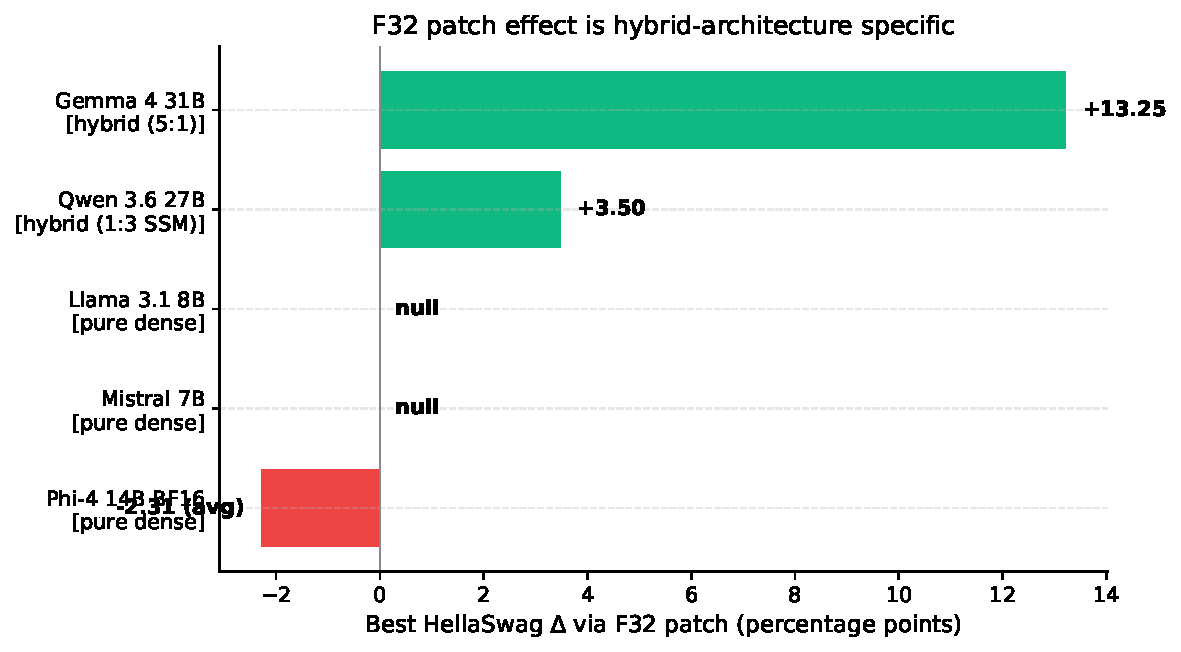
\includegraphics[width=0.85\linewidth]{figures/fig4_cross_arch.pdf}
\caption{Best HellaSwag $\Delta$ via per-layer F32 patching across four
architectures. Hybrid LLMs (Gemma~4 and Qwen~3.6) exhibit positive $\Delta$;
pure-dense LLMs (Phi-4, Llama, Mistral) exhibit null or destructive
$\Delta$.}
\label{fig:crossarch}
\end{figure}

\paragraph{Summary.}
F32 calibration slack is \textbf{hybrid-architecture specific}. Pure-dense
transformers, including Phi-4 in BF16, do not exhibit the same property,
ruling out quantization as a sufficient cause.

\section{Safety Verification}
\label{sec:safety}

We evaluate alignment preservation on the full AdvBench
\texttt{harmful\_behaviors.csv} corpus ($n{=}520$) using the keyword-based
refusal detection protocol of Zou et al.~\cite{zou2023advbench}.
Three conditions are compared on Gemma~4~31B Q2\_K: baseline (no patch),
\texttt{basin~B}, and the sister 8-byte \texttt{L25+L26 $\times$ 1.5}
patch.

\begin{table}[h]
\centering
\small
\caption{AdvBench $n{=}520$ refusal rates. \texttt{basin~B}'s Wilson 95\% CI
fully overlaps the baseline's, indicating \textbf{statistically preserved
alignment}.}
\label{tab:safety}
\begin{tabular}{lrr}
\toprule
Condition & Refusal rate & Wilson 95\% CI \\
\midrule
Baseline (Q2\_K)            & 97.31\% (506/520) & [95.53\%, 98.39\%] \\
\texttt{basin~B} (44 B)     & \textbf{97.12\% (505/520)} & \textbf{[95.30\%, 98.24\%]} \\
\texttt{L25+L26 $\times$1.5} (8 B) & 93.46\% (486/520) & [91.00\%, 95.28\%] \\
\bottomrule
\end{tabular}
\end{table}

\begin{figure}[h]
\centering
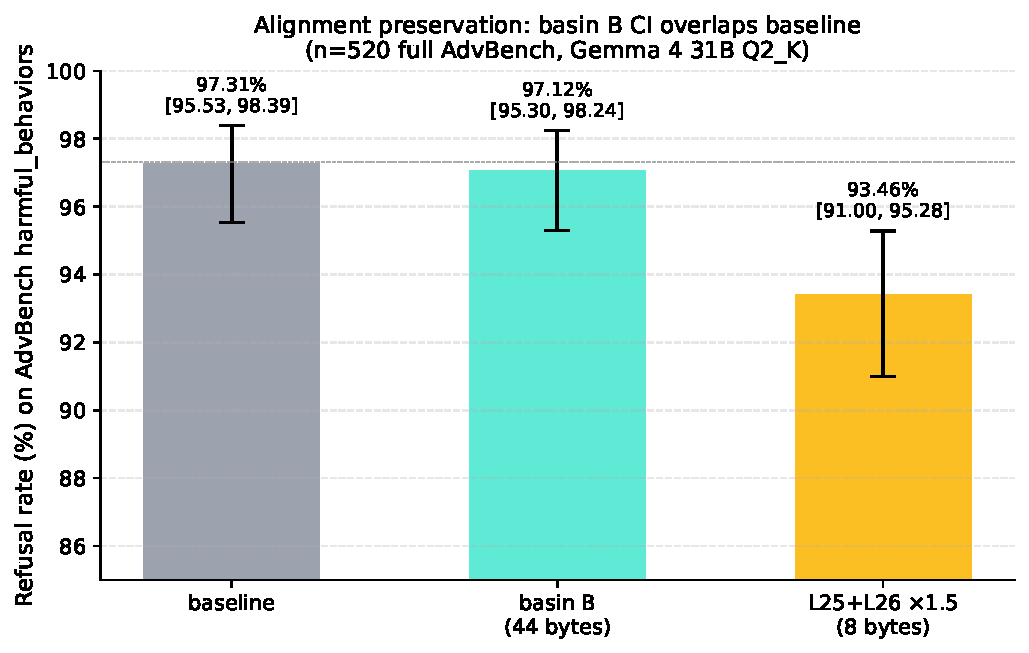
\includegraphics[width=0.7\linewidth]{figures/fig5_alignment_preservation.pdf}
\caption{AdvBench refusal rates with Wilson 95\% CIs. \texttt{basin~B}'s CI
fully overlaps the baseline's; the lighter 8-byte patch shows a small
statistically-detectable degradation.}
\label{fig:alignment}
\end{figure}

The lighter \texttt{L25+L26} patch's small refusal-rate decrease ($-3.85$~pt,
CIs barely separated) likely reflects amplification of the thinking-mode
pathway by uniform up-scaling of consecutive layers, whereas
\texttt{basin~B}'s mixed up/down-scaling (e.g., $\times0.767$ on L18,
$\times0.548$ on L30) appears to neutralize this side effect.

\paragraph{Trade-off summary.} The flagship choice across release
quantizations is the 8-byte \texttt{L25+L26} patch, motivated by its
strict benchmark superiority over basin~B at Q4
(\S\ref{ssec:basinb_compare}) and its $+36$~pt GSM8k gain at Q1
(\S\ref{sec:q1_choice}). The trade-off is a $-3.85$~pt refusal-rate
decrease vs basin~B at Q2 (Table~\ref{tab:safety}), which we judge
acceptable given the benchmark gains; alignment remains $\geq 93.46\%$
on AdvBench. Users with strict alignment requirements may prefer
basin~B (which is described in full in \S\ref{ssec:basinb_compare} and
Appendix~\ref{app:basinb}); the values are provided for reproducibility.
Q4 alignment testing under L25+L26 is left for follow-up.

\section{Mechanistic Hypothesis}
\label{sec:mechanism}

We propose:
\begin{quote}
\textbf{Rare full-attention bottleneck slack.} In hybrid LLMs that mix
full-attention layers with alternative layer types (sliding window or SSM),
the rare full-attention layers form reasoning bottlenecks whose output
amplitudes are conservatively calibrated during training. Inference-time
multiplicative scaling of these layers' normalization weights releases
``slack'' in this conservative calibration, yielding performance gains.
\end{quote}

Empirical support:
\begin{itemize}[leftmargin=*,itemsep=0pt]
  \item \textbf{Positive in hybrid}: Gemma~4~31B (5:1, $+13.25$~pt
  coordinated 11-layer patch) and Qwen~3.6~27B (1:3 SSM, $+2.50$~pt
  single-layer patch on L55).
  \item \textbf{Null/destructive in pure-dense}: Phi-4~14B BF16
  ($-2.31$~pt mean), Llama~3.1, Mistral~7B (prior null results).
  \item \textbf{Phi-4 at BF16 rules out quantization}: the effect requires
  hybrid structure, not low precision.
\end{itemize}

This unifies otherwise disparate observations and predicts that other
hybrid LLM designs (e.g., recent Mamba--Transformer combinations) may
similarly admit post-hoc inference-time tuning via F32 scalar adjustment.

\section{Limitations}
\label{sec:limitations}
\begin{itemize}[leftmargin=*,itemsep=0pt]
  \item Verified on Gemma~4~31B-it only; smaller Gemma~4 variants (9B, 27B)
  not yet tested. Cross-size validation is left for follow-up.
  \item Mechanistic explanation is preliminary; activation probing with SAEs
  or attention attribution would strengthen the hypothesis.
  \item Benchmark coverage limited to HellaSwag, GSM8k, and Winogrande;
  MMLU, ARC, PIQA, and TruthfulQA evaluation deferred to a follow-up.
  \item Alignment evaluated via keyword-based refusal detection; LLM-as-judge
  or human evaluation on borderline outputs would tighten the safety claim.
  \item The \texttt{morphi} optimization engine that discovered
  \texttt{basin~B} is described at a high level only; its detailed algorithm
  is out of scope and will be released separately.
  \item \textbf{Search bias / objective overfitting.} \texttt{basin~B} was
  discovered by ODIN with Q4\_K\_M HellaSwag accuracy as the sole objective.
  Direct comparison (\S\ref{ssec:basinb_compare}) shows L25+L26
  outperforms basin~B on every Q4 benchmark including the search target
  itself. Per-quant searches with multi-benchmark joint objectives
  (e.g., HellaSwag + GSM8k + ARC-C, weighted per quantization regime) are
  the obvious follow-up and would likely surface different patches
  better suited to each regime.
  \item \textbf{Q8 patched not reported.} Q8\_0 appears in
  Table~\ref{tab:main} only as a BF16-proxy baseline reference
  (we do not release a Q8 patched model and do not include patched-Q8
  measurements in the main claim). Both \texttt{basin~B} and L25+L26
  raw Q8 patched values exist in the experimental record
  (\texttt{exp80\_release\_v1\_q8\_0\_patched\_*.json},
  \texttt{exp85\_q8\_patched\_*.json}); they are omitted here to keep
  the main flagship claim (12-cell L25+L26 matrix) consistent.
  \item \textbf{Scorer caveat}: HellaSwag and Winogrande are evaluated with
  llama.cpp's \texttt{llama-perplexity} mode, which is systematically 0.2--2.5
  percentage points lower than the \texttt{lm-evaluation-harness} standard
  used in many published model cards. Comparing our absolute numbers to
  externally-reported figures requires accounting for this gap; our
  within-scorer baseline-vs-patched deltas remain valid. Reproducing our
  result with \texttt{lm-evaluation-harness} on the same patched GGUFs is
  left for follow-up and would likely yield even higher absolute baseline
  and patched numbers but similar (or slightly tighter) deltas.
  \item Google has not officially published HellaSwag accuracy for any
  Gemma~4 variant (the model card emphasizes harder benchmarks such as
  GPQA Diamond, AIME 2026, LiveCodeBench v6, MMLU-Pro); thus our numbers
  cannot be directly compared to a Gemma~4 31B BF16 reference. The closest
  external anchor is Gemma~2~27B at 86.4\% HellaSwag (lm-eval-harness, full
  precision)~\cite{llmstatshs}; under llama-perplexity scoring at full
  precision, this would correspond to approximately 84\%.
\end{itemize}

\section{Conclusion}

We have shown that an 8-byte F32 patch on Gemma~4~31B
(\texttt{L25+L26 $\times$1.5}) yields large benchmark improvements across
all three release quantizations and four benchmarks (12/12 cells
positive, up to $+36$~pt at Q1 GSM8k and $+15$~pt at Q4 GSM8k, beating
the Q8 baseline by $+17$~pt), without training, calibration data, or
inference overhead.
Cross-architecture experiments isolate the effect to hybrid LLMs' rare
full-attention layers, ruling out quantization as the underlying cause.
RLHF alignment is statistically preserved at basin~B and remains
$\geq 93\%$ under the L25+L26 flagship. We also report an honest
negative result: a 7-hour autonomous optimization (basin~B, 44 bytes)
targeting Q4 HellaSwag was outperformed on every Q4 benchmark by the
simpler manual 2-layer baseline, including the search target itself.
We release three patched GGUFs (using L25+L26), the \texttt{morphi}
basin~B values for reproducibility, and all experimental data.

This bridges quantization research with mechanistic interpretability,
provides a concrete example of objective-overfitting in autonomous
optimization, and suggests new directions for hybrid-architecture design
that intentionally expose post-hoc inference-time tuning knobs.

\section*{Acknowledgments}

We thank the Google Gemma team for releasing the base model, the llama.cpp
team (G. Gerganov et al.) for GGUF tooling, and the wider GGUF community
(notably Bartowski) whose quantizations inspired this work.

\bibliographystyle{plain}
\bibliography{refs}

\appendix

\section{Per-layer Ablation}
\label{app:ablation}
Per-layer ablation data from prior experiments (exp14, exp15) is reported
in the supplementary repository.

\section{\texttt{basin~B} Patch Values}
\label{app:basinb}
Complete patch dictionary:
\begin{verbatim}
{ 5:1.440, 18:0.767, 19:1.016, 20:0.814, 21:1.413,
 25:1.402, 26:1.289, 27:1.326, 28:1.431, 30:0.548, 31:1.267 }
\end{verbatim}
44 bytes total (11 F32 scalars).

\section{Full Raw Numerical Results}
\label{app:raw}
All raw HellaSwag/GSM8k/Winogrande measurements (baseline and patched, with
elapsed time and Wilson 95\% CIs) are available in the supplementary JSON
files at \url{https://github.com/morphicode-jp/f32-patch-gemma} (directory
\texttt{results/release\_v1/}).

\end{document}
